\documentclass[8pt, xcolor = dvipsnames]{beamer}



\usepackage{beamerthemesplit}
\renewcommand{\baselinestretch}{1.5}\normalsize % Zeilenabstand 1.5

% make own frame on Beginn of each section
\AtBeginSection[]{
  \begin{frame}
  \vfill
  \centering
  \begin{beamercolorbox}[sep=8pt,center,shadow=true,rounded=true]{title}
    \usebeamerfont{title}\insertsectionhead\par%
  \end{beamercolorbox}
  \vfill
  \end{frame}
}



\usepackage{caption}
\makeatletter
\newcommand\notsotiny{\@setfontsize\notsotiny{7}{7}}
\newcommand\micro{\@setfontsize\notsotiny{4.5}{4.5}}
\newcommand\middletiny{\@setfontsize\notsotiny{6}{6}}
\makeatother
\usepackage{numprint}
\npthousandsep{\,}
\usepackage{csquotes}
\usepackage{array}
\usepackage{dirtytalk}
\usepackage{amsmath}
\usepackage{bm}
\usepackage{multirow}
\usepackage{amssymb}
\usepackage{amsthm}
\usepackage{amsfonts}
\usepackage{color}
\usepackage{layouts}
% printing the textsize used
% \printinunitsof{cm}
% \prntlen{\textwidth}
\usepackage{tabularx}
\usepackage{graphicx}
\usepackage{pdfpages}
\usepackage[ngerman]{babel}

%\usetheme{default}
%\usetheme{AnnArbor}
%\usetheme{Antibes}
%\usetheme{Bergen}
%\usetheme{Berkeley}
\usetheme{Berlin}
%\usetheme{Boadilla}
%\usetheme{CambridgeUS}
%\usetheme{Copenhagen}
%\usetheme{Darmstadt}
%\usetheme{Dresden}
%\usetheme{Frankfurt}
%\usetheme{Goettingen}
%\usetheme{Hannover}
%\usetheme{Ilmenau}
%\usetheme{JuanLesPins}
%\usetheme{Luebeck}
%\usetheme{Madrid}
%\usetheme{Malmoe}
%\usetheme{Marburg}
%\usetheme{Montpellier}
%\usetheme{PaloAlto}
%\usetheme{Pittsburgh}
%\usetheme{Rochester}
%\usetheme{Singapore}
%\usetheme{Szeged}
%\usetheme{Warsaw}
%\usecolortheme[named=RoyalBlue]{structure}
\usecolortheme{seahorse}

\usepackage{listings}


\usepackage[T1]{fontenc}          % erlaubt Umlaute (Zeichenbelegung)
\usepackage[utf8x]{inputenc}     % erlaubt �-Eingabe �ber die Tastatur
\usepackage[ngerman]{babel}  
\usepackage{amsmath,amsfonts,amssymb}

\usepackage{xcolor}

%%%%%%%%%%%%%%%Foliennummerierung%%%%%%%%%%%%%%%%%%%%%%%%%%%%%%%%%%%%%%%%%
\setcounter{framenumber}{0} 
\setbeamertemplate{footline}[frame number]
%%%%%%%%%%%%%%%Foliennummerierung%%%%%%%%%%%%%%%%%%%%%%%%%%%%%%%%%%%%%%%%%

\title{Masterthesis: \textit{Multiclass}-Klassifizierung \\
 von Nachrichten Schlagzeilen}        % Titel (Kommando muss aufgerufen werden)
\author{Marc Schmieder}     % Autor(en) 
\date{06.02.2020}

\subtitle{Vergleich zwischen neuronalen Netzen und baumbasierten Algorithmen auf verschiedenen Repräsentationen von Wörtern}  % etwas kleinere Schrift als der Titel
\institute{Prof. Dr. Andreas Groll, Statistical Methods for Big Data, TU Dortmund} % Betreuer/Uni/Veranstaltung/etc.


\begin{document}                  % Ende der Pr�ambel, Beginn der Pr�sentation

\begin{frame}                     % Titelfolie
 \maketitle                       % Kommando zum Aufruf der Titelfolie
\end{frame}

%%%%%%%%Beginn%%%%%%%%%%%%%%%%%%%%%%%%%%


\tableofcontents

\section{Motivation und Zielstellung}



\begin{frame}{Motivation}

   \begin{itemize}
   \item Natural Language Processing (NLP) ist aktuelles Thema mit vielen Anwendungsfällen, zB. überwachte Klassifikation von Kurztexten.
   \item Größtenteils Artikel und Tutorials über binäre Klassifikation (zB. IMDB Sentiment Classification, Spam Vs NonSpam etc.)
   \item In der Realität oft viel mehr Klassen, zB:
   \item Themen-Kategorisierung von Kundenbeschwerden
   \item Tagging von Forenbeiträgen (Stackoverflow)
   \item Produktkategorien von Artikeln anhand Artikelbeschreibung
   \item Kategorisierung von Nachrichtenkategorien
   \end{itemize}
\end{frame}  

\begin{frame}{Zielstellung}

\begin{block}{Methodik}
\begin{itemize}
    \item \textbf{Verschiedene Repräsentation der Wörter}: (Word Embeddings): BOW, TFIDF, GloVe, SOW GloVe 
    \item \textbf{Verschiedene Machine Learning Modelle}: Baumbasierte Verfahren (XGBoost, Random Forest) VS. neuronale Netze (MLP, CNN, LSTM)
\end{itemize}{}
\end{block}{}

\begin{block}{Untersuchungsfragen}
\begin{itemize}
    \item Welche Embeddings funktionieren gut mit welchen Modellen?
    \item Wie groß sind die Unterschiede bei den vorliegenden Daten?
    \item Welchen Unterschied macht die Berücksichtigung der Reihenfolge?
    \item Was lernen die Modelle bzw. ist der Output interpretierbar?
\end{itemize}{}
\end{block}{}


\end{frame}



\section{Datensatz und Exploration}


\begin{frame}{Datensatz I}

   \begin{itemize}
   \item \textit{News Category Dataset} von Machine Learning Plattform \textit{Kaggle}, Sprache: Englisch
   \item \numprint{200853} Beobachtungen, mit Informationen  über Artikel der US-Amerikanischen Onlinezeitung \textit{Huffpost}
   \item  Veröffentlichungszeitraum: 28.01.2012 bis zum 25.05.2018 (> $6$ Jahre)
   \item Spalten: Schlagzeile, Author(en), Link zum Artikel, Kurzbeschreibung, Datum, Kategorie
   \item Kategorie ist Zielvariable ($41$ Ausprägungen), unabhängige Variable ist nur die Schlagzeile
   \end{itemize}

\end{frame}


\begin{frame}{Datensatz II}

\begin{table}[ht]
\centering
\notsotiny
\begin{tabular}{|m{1cm}||lll|}
  
  \hline
Daten\-punkt & Kategorie & Schlagzeile & Author(en)  \\ 
  \hline
1 & STYLE \& BEAUTY & Kardashians Eyewear: \dots  & Jessica Misener \\  
2 &  WELLNESS & Sports Drink Alternatives? 7  \dots & Meredith Melnick \\
3 &  STYLE \& BEAUTY & Nicole Kidman's Topless \dots & Ellie Krupnick \\
4 &  SCIENCE & Second Man On Moon Claims  \dots & Tyler McCarthy \\
5 &  ENTERTAINMENT & Popcorn Preview: House of  (2013) & Leslie Sisman \dots \\

   \hline
   \hline
Daten\-punkt & Link & Kurzbeschreibung & Datum \\
   \hline
1 & https://www.huffing \dots & What else can we photoshop \dots & 2012-08-10 \\   2 & https://www.huffing \dots & In this scenario, homemade, all \dots & 2012-06-04 \\ 
3 & https://www.huffing \dots & PHOTOS: From the very first \dots & 2014-01-10 \\ 
4 & https://www.huffing \dots & - & 2014-04-29 \\ 
5 & https://www.huffing \dots & House of Cards is a smart, s\dots & 2013-03-31 \\ 
\hline 

\end{tabular}

\caption{Ausschnitt von 4 Datenpunkten aus dem unbearbeiteten Datensatz}
\end{table}

\end{frame}  



\begin{frame}{Cleaning}
\begin{itemize}
   \item Konvertierung der Großbuchstaben zu Kleinbuchstaben (\textit{Teacher}, \textit{teacher})
   \item Ursprung aus verschiedenen Ländern: Entfernung von Sonderzeichen (\say{©} oder \say{™}), da Konvertierungsfehler bei gemischten Encodings
   \item  \say{aren't} $\xrightarrow{}$ \say{are not}, \say{he'll} $\xrightarrow{}$ \say{he will},  \say{here's} $\xrightarrow{}$ \say{here is} 
   \item \say{trump's} $\xrightarrow{}$ \say{trump his}, dann \say{john's son} $\xrightarrow{}$ \say{john its son}
   \item Entfernung von leeren Texten (6 Beobachtungen). Insgesamt \numprint{200847} Beobachtungen verbleibend.
   \end{itemize}
\end{frame}



\begin{frame}{Zusammenlegung der Kategorien I}

   \begin{itemize}
   \item Namentliche und inhaltliche Ähnlichkeit der Kategorien (\textit{arts \& culture} und \textit{culture \& arts})
   \item Schwierig mit menschlicher Intuition auseinander zu halten.
   \item Reduktion auf $32$ Kategorien (ab $0.50$, zuzüglich \textit{arts \& culture} \textit{arts})
   \end{itemize}
 
 \begin{table}[ht]
\begin{center}
\notsotiny
\begin{tabular}{ | p{0.1 \textwidth} | p{0.42 \textwidth}| p{0.42 \textwidth} | }
  \hline
Beispiel & Kategorie \textit{parents}  & Kategorie \textit{parenting} \\ 
  \hline
1 & 40 tweets that sum up life with 4-year-olds & a baby book of disasters \\ 
  2 & these were the trendiest baby names in the late '80s & it is time to find your tribe \\ 
  3 & these quotes from kids are hilarious, adorable and oddly insightful & help huffpost parents win a webby award! \\ 
  4 & 30  'star wars'-inspired names parents are giving their babies & why our 'imperfect' moments are perfect to our children \\ 
   \hline
\end{tabular}
\caption{Beispiele für Schlagzeilen der Kategorien \textit{parents} und \textit{parenting}}
\label{tab:parentsMerge}
\end{center}
\end{table}
 
\end{frame}
 
 
\begin{frame}{Zusammenlegung der Kategorien II}

\begin{table}[ht]
\begin{center}
\notsotiny
\begin{tabular}{|l|l|c|c|}

  \hline
Kategorie 1 & Kategorie 2  & relative Schnittmenge & neue Kategorie\\
  \hline
\textit{healthy living} & \textit{wellness} & 0.76 & \textit{wellness \& healthy living} \\ 
  \textit{parents} & \textit{parenting} & 0.74 & \textit{parents} \\ 
  \textit{taste} & \textit{food \& drink} & 0.70 & \textit{food, drink \& taste}\\ 
   \vdots & \vdots & \vdots & -\\
  \textit{fifty} & \textit{parenting} & 0.50 & -\\ 
    \vdots & \vdots & \vdots & -\\
  \textit{parents} & \textit{fifty} & 0.48 & - \\ 
  \textit{arts \& culture} & \textit{arts} & 0.46 & \textit{arts \& culture}\\  
  \vdots & \vdots & \vdots & -\\

  \textit{crime} & \textit{food \& drink} & 0.04 & -\\
  \hline 
  \hline 
  \multicolumn{2}{|c|}{Mittelwert} &  0.24 & \\
   \hline
\end{tabular}
\caption{Relative Schittmenge der $100$ häufigsten Wörter für Paare an Kategorien}
\label{tab:categoryMerge}
\end{center}
\end{table}
   
\end{frame}   





\begin{frame}

\begin{figure}[ht]
    \centering
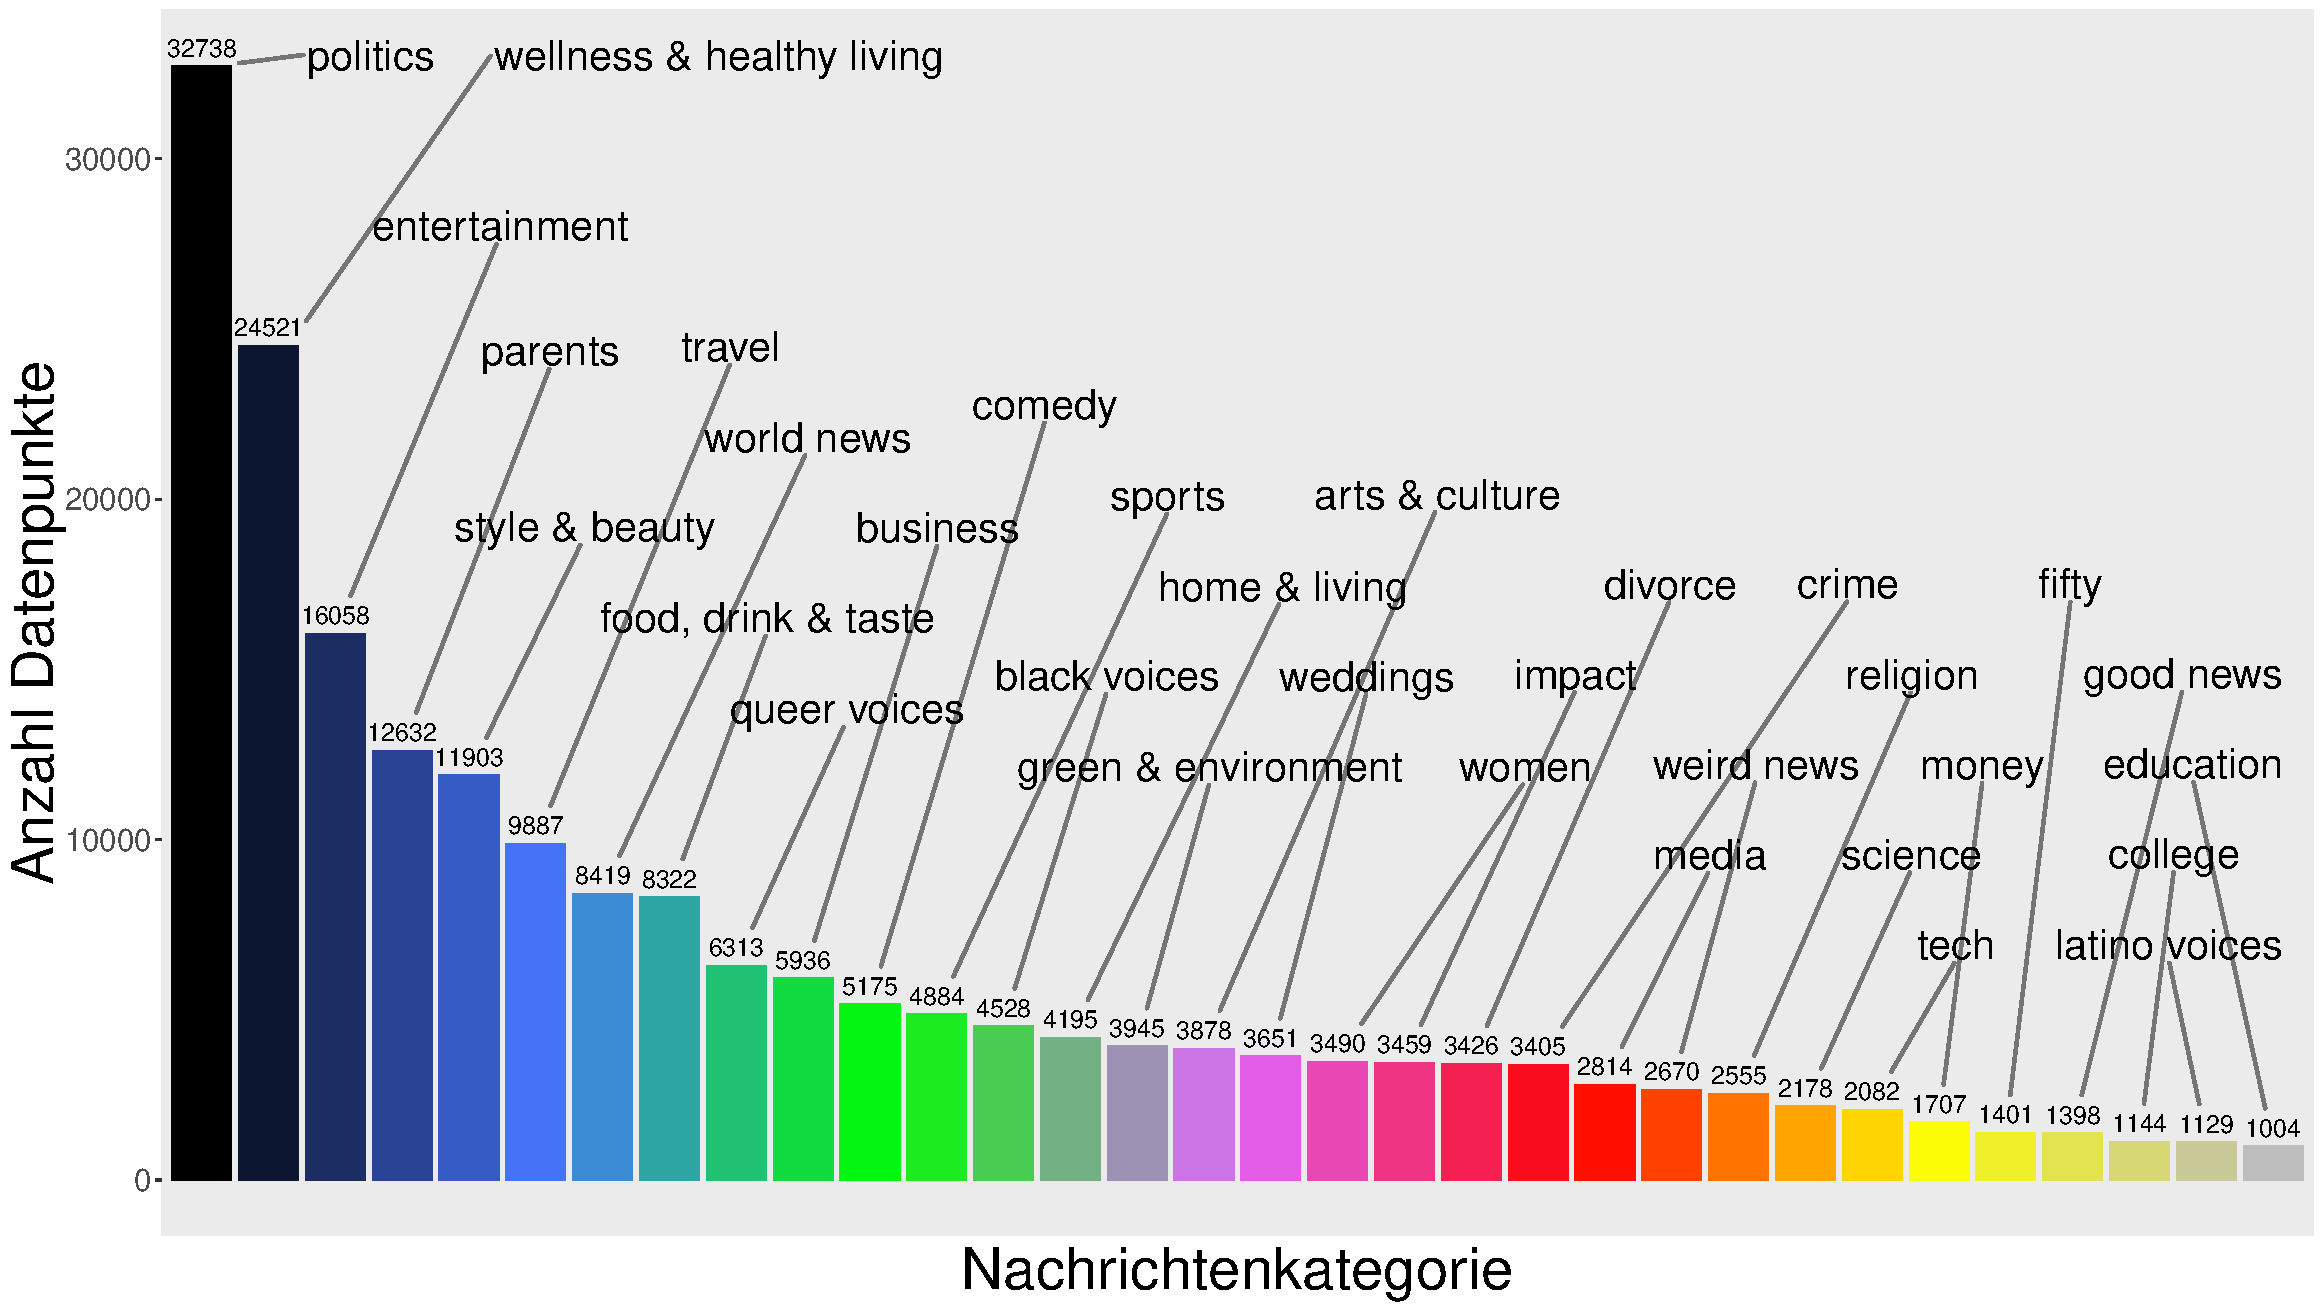
\includegraphics[width = \textwidth,  keepaspectratio]{Images/barplotCategories.pdf} 
\caption{Anzahl Datenpunkte pro Nachrichtenkategorie}
\label{abb:barplotCategories}
\end{figure}

\end{frame}





\begin{frame}
\begin{figure}[ht]
    \centering
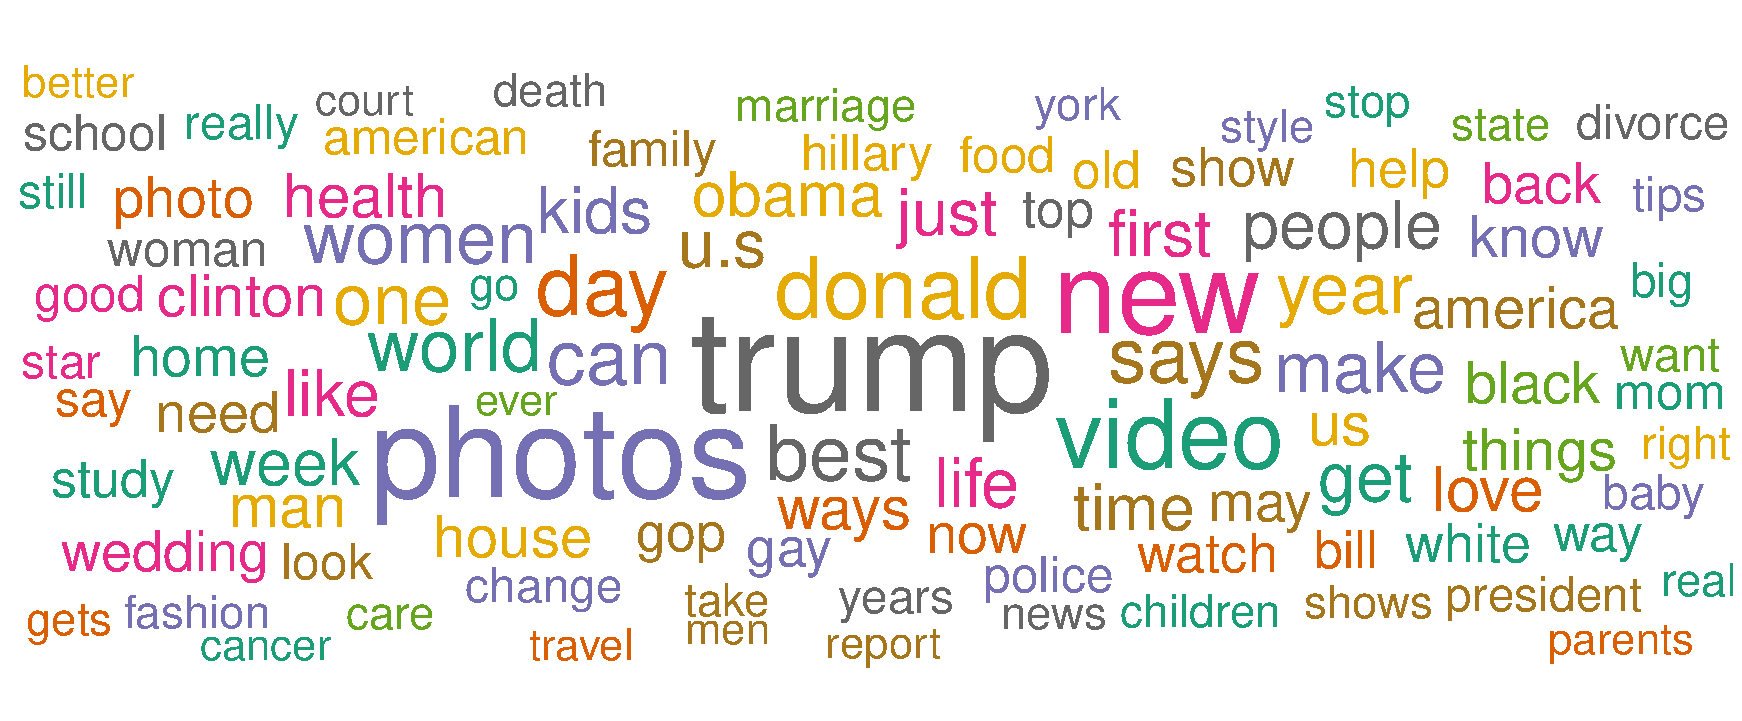
\includegraphics[width = \textwidth,  keepaspectratio]{Images/wordCloudAll.pdf} 
\caption{\textit{wordcloud} für die häufigsten 100 Wörter aller Kategorien}
\label{abb:WordcloudAll}
\end{figure}
\end{frame}


\section{Repräsentation der Wörter}



\begin{frame}{Bag-Of-Words}

\begin{block}{Vorauswahl}
In einer Vorauswahl wurden viele Repräsentation der Wörter getestet, hier werden die Word-Embeddings der Endauswahl vorgestellt
\end{block}{}

\begin{table}[ht]
\begin{center}

\begin{tabular}{|c||ccccccccccc|}
\hline
\multicolumn{12}{|c|}{\textit{BOW} \textit{dtm}} \\
\hline 
   Satz   & the & dog & cat & like & likes &  to & sit  & owner & his &  does & not \\
      \hline
Satz 1 & $1$ & $0$ & $1$ & $0$ & $1$ & $1$ & $1$ & $0$ & $0$ &  $0$ & $0$ \\
Satz 2 & $1$ & $1$ & $0$ & $1$ & $0$ & $0$ & $0$ & $1$ & $1$ &  $1$ & $1$ \\
Satz 3 & $0$ & $1$ & $0$ & $0$ & $1$ & $0$ & $0$ & $1$ & $0$ &  $0$ & $0$ \\

\hline

\end{tabular}
\end{center}{}
\caption{Beispiel für eine \textit{document-term-matrix} für die $3$ Beispielsätze \textit{the cat likes to sit}, \textit{the dog does not like his owner}, \textit{the owner likes the dog} jeweils für das \textit{BOW Embedding}}  
\label{tab:BOWExample}

\end{table}
\end{frame}{}

\begin{frame}{GloVe: Global Word Vektors}


\begin{itemize}
    \item Methode zur Repräsentation von Wörtern im $F$- dimensionalen Raum.
    \item Datenpunkt ist Sequenz aus Wort Vektoren und hat Matrix-Form mit Dimension $F \times maxWords$
    \item Unüberwachtes Lernen der Vektoren
    \item \textbf{Möglichkeit 1:} Training auf eigenem Textkorpus
    \item \textbf{Möglichkeit 2:} Vortrainierte Datensätze auf Wikipedia (GloVe 50D) oder genereller Internet Crawl (Glove 300D)
\begin{block}{Weiteres Embedding:}
Bilde normierte Summen aus Wortvektoren und bilde so die Repräsentation des Satzes durch einen Vektor der Dimension $F$
\end{block}{}
\begin{block}{Ähnliches Embedding:}
Überwachtes Lernen der Wortvektoren durch eine \textit{embedding}-Zwischenschicht mit $F$ Neuronen im Neuronalen Netz
\end{block}{}

\end{itemize}{}

\end{frame}{}

\begin{frame}{GloVe Beispiel}
\begin{table}[ht]
\micro
\centering
\begin{tabular}{|m{0.6cm}m{0.4cm}m{0.4cm}m{0.4cm}m{0.4cm}m{0.4cm}m{0.4cm}m{0.4cm}m{0.4cm}m{0.4cm}m{0.4cm}m{0.4cm}m{0.4cm}m{0.4cm}m{0.4cm}m{0.4cm}m{0.4cm}m{0.4cm}m{0.4cm}m{0.4cm}m{0.4cm}m{0.4cm}m{0.4cm}m{0.4cm}m{0.4cm}m{0.4cm}m{0.4cm}|}
  \hline
 & reese & wither\-spoon & had & the & ' & snl & ' & cast & apolo\-gize & to & their & moms & -- & -- & -- & -- & -- & -- & -- & -- & -- & -- & -- & -- & -- & -- \\ 
  \hline
Dim 0 & -0.42 & -0.49 & 0.60 & 0.42 & -0.04 & -0.31 & -0.04 & 0.02 & -0.02 & 0.68 & 0.42 & 0.05 & 0.00 & 0.00 & 0.00 & 0.00 & 0.00 & 0.00 & 0.00 & 0.00 & 0.00 & 0.00 & 0.00 & 0.00 & 0.00 & 0.00 \\ 
  Dim 1 & -0.00 & 0.35 & -0.52 & 0.25 & 1.20 & -0.20 & 1.20 & 0.42 & -0.55 & -0.04 & 0.13 & 0.40 & 0.00 & 0.00 & 0.00 & 0.00 & 0.00 & 0.00 & 0.00 & 0.00 & 0.00 & 0.00 & 0.00 & 0.00 & 0.00 & 0.00 \\ 
  Dim 2 & -0.37 & -0.50 & 0.41 & -0.41 & 0.35 & -0.09 & 0.35 & 0.41 & -0.25 & 0.30 & -0.06 & 0.16 & 0.00 & 0.00 & 0.00 & 0.00 & 0.00 & 0.00 & 0.00 & 0.00 & 0.00 & 0.00 & 0.00 & 0.00 & 0.00 & 0.00 \\ 
  Dim 3 & 0.10 & 0.07 & -0.37 & 0.12 & -0.56 & 0.74 & -0.56 & -0.13 & -0.26 & -0.18 & -0.57 & -0.95 & 0.00 & 0.00 & 0.00 & 0.00 & 0.00 & 0.00 & 0.00 & 0.00 & 0.00 & 0.00 & 0.00 & 0.00 & 0.00 & 0.00 \\ 
  Dim 4 & 0.54 & 0.35 & 0.37 & 0.35 & -0.52 & 0.26 & -0.52 & 0.58 & -0.04 & 0.43 & 0.50 & 0.37 & 0.00 & 0.00 & 0.00 & 0.00 & 0.00 & 0.00 & 0.00 & 0.00 & 0.00 & 0.00 & 0.00 & 0.00 & 0.00 & 0.00 \\ 
  Dim 5 & 0.08 & 0.42 & 0.61 & -0.04 & -0.67 & -0.21 & -0.67 & 1.18 & 0.18 & 0.03 & 0.21 & 0.51 & 0.00 & 0.00 & 0.00 & 0.00 & 0.00 & 0.00 & 0.00 & 0.00 & 0.00 & 0.00 & 0.00 & 0.00 & 0.00 & 0.00 \\ 
  \vdots & \vdots & \vdots & \vdots & \vdots & \vdots & \vdots & \vdots & \vdots & \vdots & \vdots & \vdots & \vdots & \vdots & \vdots & \vdots & \vdots & \vdots & \vdots & \vdots & \vdots & \vdots & \vdots & \vdots & \vdots & \vdots & \vdots \\
  Dim 45 & -0.11 & -0.68 & -0.25 & -0.44 & 0.44 & 0.02 & 0.44 & -0.62 & 0.56 & -0.20 & 0.24 & 0.56 & 0.00 & 0.00 & 0.00 & 0.00 & 0.00 & 0.00 & 0.00 & 0.00 & 0.00 & 0.00 & 0.00 & 0.00 & 0.00 & 0.00 \\ 
  Dim 46 & 0.46 & 0.25 & -0.48 & 0.19 & -0.06 & -1.25 & -0.06 & 0.16 & 0.11 & 0.08 & -0.19 & 0.16 & 0.00 & 0.00 & 0.00 & 0.00 & 0.00 & 0.00 & 0.00 & 0.00 & 0.00 & 0.00 & 0.00 & 0.00 & 0.00 & 0.00 \\ 
  Dim 47 & 0.27 & 0.42 & -1.04 & 0.00 & -0.43 & 0.68 & -0.43 & -0.57 & -1.25 & -0.09 & -0.22 & 0.12 & 0.00 & 0.00 & 0.00 & 0.00 & 0.00 & 0.00 & 0.00 & 0.00 & 0.00 & 0.00 & 0.00 & 0.00 & 0.00 & 0.00 \\ 
  Dim 48 & -0.51 & -1.05 & -0.15 & -0.18 & -0.08 & 0.71 & -0.08 & -0.64 & 0.93 & -0.07 & -0.12 & 0.08 & 0.00 & 0.00 & 0.00 & 0.00 & 0.00 & 0.00 & 0.00 & 0.00 & 0.00 & 0.00 & 0.00 & 0.00 & 0.00 & 0.00 \\ 
  Dim 49 & -1.02 & -0.74 & -0.22 & -0.12 & 0.49 & -0.42 & 0.49 & -0.25 & 0.00 & -0.06 & -0.34 & 0.02 & 0.00 & 0.00 & 0.00 & 0.00 & 0.00 & 0.00 & 0.00 & 0.00 & 0.00 & 0.00 & 0.00 & 0.00 & 0.00 & 0.00 \\ 
  Dim 50 & 0.69 & 0.61 & -0.60 & -0.79 & 0.09 & 1.69 & 0.09 & 0.10 & 0.51 & -0.26 & -0.87 & 0.66 & 0.00 & 0.00 & 0.00 & 0.00 & 0.00 & 0.00 & 0.00 & 0.00 & 0.00 & 0.00 & 0.00 & 0.00 & 0.00 & 0.00 \\ 
   \hline
\end{tabular}
\caption{GloVe Embedding eines Beispieldatenpunkts: Der Satz \textit{reese witherspoon had the 'snl' cast apologize to their moms}}

\end{table}

    
\end{frame}{}




\section{Machine Learning Modelle}

\begin{frame}{Verfahren}
\begin{block}{Vorauswahl}
In einer Vorauswahl wurden viele Modelle getestet, hier werden die Modelle der Endauswahl kurz vorgestellt:
\end{block}{}

\begin{itemize}

    \item XGBoost: Baumbasiertes-Boosting Verfahren
    \item MLP: Multi-Layer Perceptron: Reguläres Feed-forward neuronales Netz
    \item CNN: Convolutional Neural Network
    \item Bi-LSTM: Bidirectional Long-Short-Term-Memory Neural Network
   
\end{itemize}
\end{frame}


\begin{frame}{XGBoost}
    \begin{itemize}
    \item Populär durch Kaggle-Wettbewerbs-Siege
        \item Wald aus Klassifikationsbäumen
        \item Boosting Verfahren: Schwierige zu klassifizierende Beobachtungen werden höher gewichtet in den sukzessiven Trainingsschritten
        \item Extrem schnelle Rechenzeit (Sparse Matrizen, BOW)
        \item Viele Libraries zum Explaining (zB. XGBoostExplainer)
    \end{itemize}{}
\end{frame}{}





\begin{frame}{Multi Layer Perceptron}
\begin{columns}[T] % align columns
\begin{column}{.48\textwidth}

\begin{itemize}
    \item Reguläres \textit{feed-forward} fully connected neuronales Netz
    \item $32$ Neuronen in der Ausgangsschicht + Softmax Aktivierungsfunktion (gilt auch für alle folgende Netze
    \item Implementation mit \texttt{keras} und Nutzung von \textit{early stopping} (gilt für alle Netze)
\end{itemize}{}

\end{column}%
\hfill%
\begin{column}{.48\textwidth}

\centering
\includegraphics[width = 6cm,  keepaspectratio]{Images/MLPScreen_DeepLearningEssentials2.PNG}
\caption{\textit{fully-connected feed-forward} Netz mit 2 Zwischenschichten}

\end{column}%
\end{columns}

\end{frame}{}





\begin{frame}{Convolutional Neural Net}
\begin{itemize}
    \item Ursprünglich zur Bilderkennung entwickelt
    \item Auch für \textit{NLP} verwendbar
    \item Gitterförmige Filter lernen Gewichte, die bei Wort-Tupeln oder Wort-Tripeln eine hohe Convolution erzeugen
\end{itemize}{}  

\begin{figure}[!ht]
\begin{center}
\includegraphics[width = 0.8\textwidth,  keepaspectratio]{Images/CNN_NLP.PNG}
\caption{Architektur eines \textit{CNN} für einen NLP Anwendungsfall}
\label{abb:CNN_NLP}
\end{center}
\end{figure}
\end{frame}{}

\begin{frame}{Long-Short-Term-Memory Neural Net}
\begin{itemize}
  \item Sehr populär für \textit{NLP} Anwendung
  \item Weiterentwicklung des Recurrent Neural Net
  \item Dateninput werden sequenziell ins Netz eingegeben
  \item Internes \say{Langes} Kurzzeitgedächnis
\end{itemize}{}  

    \begin{figure}[!ht]
\begin{center}
\includegraphics[width = 0.8\textwidth,  keepaspectratio]{Images/RNN_Example_DeepNLPpage128.PNG}
\caption{\textit{RNN} Model bei Input des Satzes: Sachin is a great }
\label{abb:RNNExample}
\end{center}
\end{figure}
\end{frame}{}

\section{Auswertung}

\begin{frame}{Framework}
\begin{itemize}
    \item Einteilung der \numprint{200847} Beobachtungen des gesamten Datensatzes in Trainings-, Test- und Validierungsdaten \item Testdaten $\numprint{20005}$ Beobachtungen, etwa 10 Prozent (Erwartungsgemäß $100$ in der kleinsten Kategorie)
    \item Von den $90$ Prozent der Daten, Stichprobe von $10$ Prozent gezogen ($9$ Prozent der gesamten Daten). $\numprint{18084}$ Beobachtungen
    \item Davon $80$ Prozent Trainingsdaten der Vorauswahl ($\numprint{14467}$ Datenpunkte) und $20$ Prozent  Validierungsdaten der Vorauswahl ($\numprint{3617}$ Datenpunkte)
    \item Tuning und Struktur der Netze auf Validierungsdaten
\end{itemize}{}
\end{frame}{}


\begin{frame}{Finale Auswahl und Evaluation}

\begin{table}[ht]
\notsotiny
\centering
\begin{tabular}{|l||ccccc|}
  \hline
\textit{Embedding}, Modell & $accuracy$ & $\overline{accuracy}$ & $fscore_M^{(1)}$ & $CE$ & $\bar{p}_{IfCorrect}$ \\ 
  \hline
\textit{BOW, XGBoost} & \textcolor{red}{0.624} & 0.487 & 0.541 & \textcolor{red}{1.447} & 0.653 \\ 
  \textit{GloVe 300D, CNN} & 0.668 & 0.521 & 0.562 & 1.247 & \textcolor{red}{0.646} \\ 
  \textit{GloVe 300D, Bi-LSTM} & \textcolor{ForestGreen}{0.689} & \textcolor{ForestGreen}{0.552} & \textcolor{ForestGreen}{0.587} & \textcolor{ForestGreen}{1.124} & \textcolor{ForestGreen}{0.825} \\ 
  \textit{SOW GloVe 300D, MLP} & 0.625 & \textcolor{red}{0.455} & \textcolor{red}{0.499} & 1.358 & 0.705 \\ 
   \hline
\end{tabular}
\label{tab:finalSelection}
\caption{Evaluation der Modelle der finalen Auswahl bezüglich der Gütemaße $accuracy$, $\overline{accuracy}$, $fscore_M^{(1)}$, $CE$ und  $\bar{p}_{IfCorrect}$}
\end{table}


\small{
\begin{align*}
&accuracy = \frac{\sum_{i=1}^C tp_i}{N}, & &\overline{accuracy} = \frac{1}{C} \sum_{i = 1}^C accuracy_{C_i}  \\
&fscore_{M}^{(1)} = \frac{2 \cdot precision_{M} \cdot recall_{M}}{precision_{M} + recall_{M}} & &\Biggl(precision_M = \frac{\sum_{i = 1}^C \frac{tp_i}{tp_i + fp_i} }{C} \hspace{0.5cm} recall_M = \frac{\sum_{i = 1}^C \frac{tp_i}{tp_i + fn_i} }{C}\Biggr)\\
&CE = - \frac{1}{N}\sum_{i=1}^N \sum_{j = 1}^C y_{ij} log(p_i(c_j))  & &\bar{p}_{IfCorrect} = \frac{1}{N}\sum_{i=1}^N  I_{\{\hat{y}(x_i) = y_i\}} p(x_i = y_i) 
\end{align*}
}

    
\end{frame}{}




\begin{frame}
\begin{figure}[ht]
    \centering
\includegraphics[width = \textwidth,  keepaspectratio]{Images/FinalSelectionAccByClass.pdf} 
\caption{\textit{accuracy} je Kategorie für die $4$ Modelle der Endauswahl. Geordnet absteigend von links nach rechts nach Größe der Kategorie im Testdatensatz}
\label{abb:AccByClass}
\end{figure}
\end{frame}

\begin{frame}
\begin{itemize}
    \item \textit{XGBoost} schneidet in $14$ Kategorien am schlechtesten ab und in keiner am besten.
     \item \textit{CNN} dominiert $8$ Kategorien, insbesondere die beiden kleinsten \textit{college} und \textit{education}.
    \item \textit{Bi-LSTM} dominiert $19$ von $32$ Kategorien und ist in keiner am schlechtesten.
    \item \textit{MLP} performt am besten in \textit{sports}, belegt aber in $16$ der $32$ Sparten den letzten Platz. Schneidet besonders bei den $5$ kleinsten Kategorien schlecht ab. In  \textit{fifty} $0$ Prozent $accuracy$.
    \item Die $2$ größten Kategorien \textit{politics} und \textit{wellness \& healthy living} sowie \textit{divorce} und \textit{tech} werden von  allen Modellen etwa gleich gut vorhergesagt.
    \item kleine Kategorien schneiden tendenziell schlechter ab, die $7$ größten Kategorien haben in den besten Modellen eine $accuracy$ von $0.76- 0.86$ Prozent.
\end{itemize}{}
\end{frame}{}







\begin{frame}
\begin{figure}[ht]
    \centering
\includegraphics[width = \textwidth,  keepaspectratio]{Images/FinalSelectionCompareProbVsAcc.pdf} 
\caption{Anteil korrekt klassifizierter Beobachtungen für Intervalle der Modellwahrscheinlichkeiten der $4$ Modelle der Endauswahl}
\label{abb:CompareProbVsAcc}
\end{figure}
\end{frame}


\begin{frame}
\begin{itemize}
    \item \textit{Bi-LSTM}: Sicherheit zu groß
    \item \textit{CNN}, \textit{XGBoost} häufig größerer Anteil korrekt klassifizierter Beobachtungen bei geringerer Sicherheit
    \item \textit{MLP} Tendenziell genau so sicher, wie auch korrekt
\end{itemize}{}
\end{frame}{}


\section{Fazit und weitere Schritte}

\begin{frame}
\begin{block}{Zusammenfassung}
\begin{itemize}
    \item Bi-LSTM dominiert mit $68.9$ Prozent $accuracy$
    \item traditionelle Embeddings performen solide
\end{itemize}{}
\end{block}

\begin{block}{Weitere Analysen}
\begin{itemize}
\item Visualisierung der Filtern des CNN
\item Erklärung von einzelnen Beobachtungen von BOW, XGBoost mit Waterfall-Grafik (XGBoostExplainer)
\item BOW, XGBoost Variablenwichtigkeiten in Wordclouds
\item Ideen für Bi-LSTM und Sums-of-Words Embedding?
\end{itemize}{}
\end{block}{}

\end{frame}{}

\begin{frame}
\centering
    \Large{Vielen Dank für die Aufmerksamkeit!}
\end{frame}{}

\end{document}